\section{Choice of Gesture Recognizer}
\label{sec:analysis:choice-of-gesture-recognizer}

There are two primary methods for performing gesture recognition~\cite[pp. 19-21]{prespecialisation}:

\begin{itemize}
\item Camera based
\item Motion based
\end{itemize}

Examples of camera based approaches for gesture recognition includes the use of one or more Microsoft Kinects that record the users motions~\cite{caon2011context}. The benefit of Microsoft Kinects is, that they can potentially record gestures performed with any part of the body. Another approach is an infrared gesture pendant worn by the user which records their hand motions when gestures are performed in front of their chest~\cite{starner2000gesture}.

As stated in \Cref{sec:related-work} we opt to not use camera based methods as they require a line of sight between the user and any device he intends to interact with or optionally, a line of sight between the user and multiple cameras installed in his smart home.

Hence we elected to use a motion-based approach. As of spring 2016 a significant amount (55\%) of wrist-worn wearables contained an accelerometer~\cite[pp. 2-3]{prespecialisation} and as such it makes sense to focus on motion-based gesture recognition utilizing an accelerometer.

While it is natural to use hands to perform gestures, we chose to look at wearables that are worn on the wrist rather than wearables that are worn on the hands, \eg the fingers. As shown in \Cref{fig:wearables-placement} only very few wearables are worn on the hands and we found it more interesting to develop for more widely available devices. In regards to gestures, the primary difference between recognizing a gesture with a wearable worn on the hand and on the wrist, is that the motions must be larger, when the wearable is worn on the wrist, \ie the user must move the entire arm in order to produce significant accelerations on the axes of the accelerometer.

\begin{figure}[!htb]
  \centering
  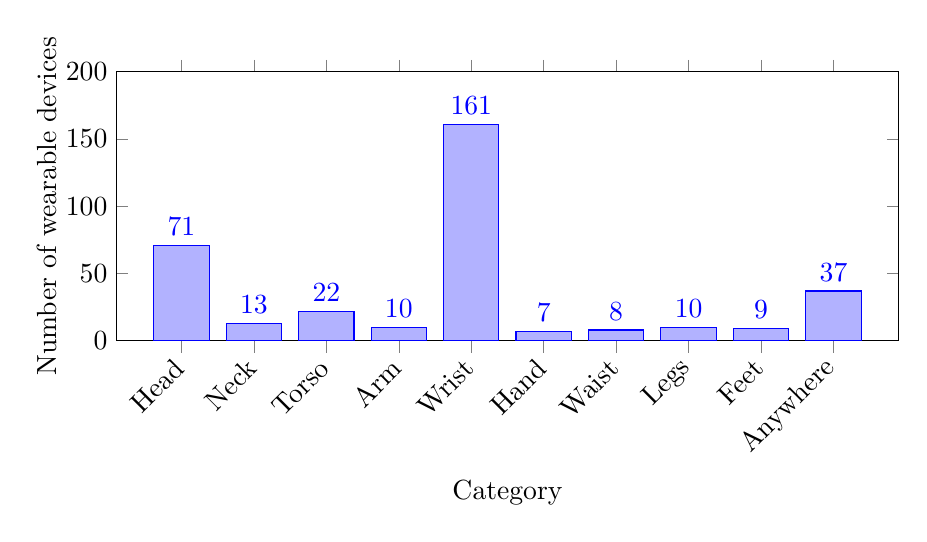
\begin{tikzpicture}
    \begin{axis}[
        height=5cm,
        width=0.95\textwidth,
        xlabel={Category},
        xticklabel style={rotate=45, anchor=east, yshift=-0.5ex},
        ylabel={Number of wearable devices},
        yticklabel style={align=right,inner sep=0pt,xshift=-0.3em},
        nodes near coords align={vertical},
        nodes near coords,
        xtick=data,
        symbolic x coords={Head,Neck,Torso,Arm,Wrist,Hand,Waist,Legs,Feet,Anywhere},
        ybar,
        ymax=200,
        ymin=0,
        bar width=20pt,
        ]
        \addplot coordinates {(Head,71) (Neck,13) (Torso,22) (Arm,10) (Wrist,161) (Hand,7) (Waist,8) (Legs,10) (Feet,9) (Anywhere,37)};
    \end{axis}
\end{tikzpicture}
  \caption{Placements of wearables. Graph from~\cite[p. 2]{prespecialisation}, data from \protect\cite{LISTOFWEARABLES}.}
\label{fig:wearables-placement}
\end{figure}

In~\cite{prespecialisation} we used the \$3 recognizer~\cite{threedollar} which is based on the \$1 recognizer~\cite{wobbrock2007gestures}.
Both are designed to be simple and easy to implement and the main difference between them is that \$1 is designed for two-dimensional gestures drawn on a screen whereas \$3 is designed for three-dimensional gestures captured using a tri-axis accelerometer.

While the \$3 gesture recognizer works adequately~\cite[p. 55]{prespecialisation}, we decided to search for an alternative that would possibly work better on embedded and resource constrained devices.

We have the following requirements for the gesture recognizer.

\begin{itemize}
    \item It must utilize an accelerometer to detect gesture motion data.
    \item It must run on Android Wear.
    \item It must recognize a gesture faster than 200 milliseconds.
    \item It must support userdefined gestures.
    \item Preferably it should run on the wearable independently from the smartphone.
\end{itemize}

Based on these criteria we will examine the following gesture recognition solutions:

\begin{itemize}
    % \item GRT~\cite{gillian2011gesture, gillian2014gesture, gilliangesturegithub}
    \item \$3~\cite{threedollar}
    \item 1\textcent~\cite{herold20121}
\end{itemize}

% The Kiwi\footnote{For more information about Kiwi, refer to http://kiwi.ai/} and FocusMotion\footnote{For more information about FocusMotion, refer to http://focusmotion.io/} gesture recognizers were not taken into consideration as they are commercial and potentially expensive solutions and as per the requirement specification presented, we desire to use inexpensive software.

% \subsection{GRT}

% GRT, short for Gesture Recognition Toolkit, is a C++ libary for real-time gesture recognition, thus the library has support for continuous recognition of gestures. 

% The library supports various algorithms for classification of gestures, including but not limited to Naive Bayes and K-Nearest Neighbor. Furthermore the library has built in support for pre-processing of accelerations from the accelerometer as well as post-processing of classified gestures and as the library performs continuous recognition, part of the post-processing may be to timeout the receognizer after a gesture is recognizer in order to avoid recognizing multiple gestures right after each other.

% GRT works with any N-dimensional floating point vector and as such, can work with accelerometer data.

\subsection{\$3}

The \$3 gesture recognizer is based on the \$1 gesture recognizer but works with three-dimensional accelerometer measurements instead of two-dimensional coordinates~\cite{threedollar}.

The \$3 gesture recognizer translates measurements on a tri-axis accelerometer to coordinates by using the first measurement as origo and adding the difference between subsequent measurements to form a timeseries of acceleration deltas as shown in \Cref{eq:acceleration-timeseries}.

\begin{figure}[h]
\[ T = \{p_1,\ldots,p_X\} \text{ s.t. } p_i=a_i-a_{i-1} \]
\caption{Gesture trace representation in \$3. $T$ is the gesture trace, $a_i$ is an accelerometer measurement and $X$ is the number of accelerations measured.}
\label{eq:acceleration-timeseries}
\end{figure}

This timeseries $T$ is known as the gesture trace and will be rotated to find the smallest distance to the trained gesture templates.
The way \$3 works is elaborated in \Cref{sec:design:gesture-recognition}.

The gesture recognizer was used in~\cite{prespecialisation} and was found to have a precision between 58\% - 98\%, depending on the user utilizing the recognizer~\cite[p. 344]{threedollar}. The concrete implementation of the recognizer was also found to have memory issues where allocated memory was not deallocated~\cite[p. 54]{prespecialisation}.

\subsection{1\textcent}

Like the \$3 gesture recognizer, the 1\textcent gesture recognizer is also based on \$1. Where \$3 improves \$1 by adding support for a third dimension as well as use of accelerometer data, 1\textcent improves \$1 by decreasing the amount of computations, thus making it more suitable for embedded and resource constrained devices.

1\textcent decreases the amount of computations by not rotating a gesture trace when matching it with trained gesture templates. Instead it computes distances from each point in the gesture trace to the centroid of the trace as shown in \Cref{eq:one-cent-trace}.
Further description of how 1\textcent works and is used can be found in \Cref{sec:design:gesture-recognition}.

\begin{figure}[h]
\[ d = \{d_i,\ldots,d_N\} \text{ s.t. } d_i=||p_i-c|| \]
\caption{Gesture trace representation in 3\textcent. $d$ is the gesture trace represented as distances to the centroid, $p_i$ is a point in the trace and $c$ is the centroid of the trace. Source: \cite{herold20121}}
\label{eq:one-cent-trace}
\end{figure}

\subsection{Conclusion}

Concrete implementations of \$3 and 1\textcent are available and both support the Android Wear platform, although only \$3 utilizes the accelerometer data in order to train and recognize gestures. While we have previous experience with the \$3 algorithm and found it to have an accuracy of up to 98\%, we chose to utilize the 1\textcent as it requires fewer computations by not rotatiing the trace and is thus better suited for embedded devices.

The 1\textcent gesture recognizer only supports recognition in two dimensions, \eg recognition on a touch screen, therefore we choose to implement support for a third dimension and use it with accelerations on the X, Y and Z axes provided by the accelerometer of an Android Wear device by merging it with the technique used in \$3.

%%% Local Variables:
%%% mode: latex
%%% TeX-master: "../../master"
%%% End:
